% Clift: Lifting C into Lean 4 for Formal Verification
% Compile with: latexmk -lualatex clift.tex

\documentclass[sigconf,nonacm,screen]{acmart}

\usepackage{fontspec}
\usepackage{booktabs}
\usepackage{xcolor}
\usepackage{url}
% Git SHA injected at build time — generated by Justfile
\usepackage{catchfile}
\CatchFileDef{\gitsha}{gitsha.tex}{\endlinechar=-1}

% Override acmart footer to include git SHA
\AtBeginDocument{%
  \fancyfoot[R]{\footnotesize\texttt{git:\gitsha}}%
}

\usepackage{tikz}
\usepackage{pgfplots}
\pgfplotsset{compat=1.18}
\usepackage{listings}

\lstset{
  basicstyle=\ttfamily\small,
  keywordstyle=\bfseries\color{blue!70!black},
  commentstyle=\itshape\color{green!50!black},
  stringstyle=\color{red!60!black},
  breaklines=true,
  columns=flexible,
  frame=single,
  framerule=0.4pt,
  xleftmargin=1em,
  xrightmargin=0.5em,
  aboveskip=0.8em,
  belowskip=0.8em,
  numbers=none,
}

\lstdefinelanguage{Lean}{
  morekeywords={theorem,lemma,def,where,by,sorry,simp,omega,intro,apply,
    exact,have,let,if,then,else,match,with,do,return,fun,structure,class,
    instance,open,namespace,end,import,noncomputable,local,irreducible,
    attribute,section,variable,inductive,Prop,Type,Sort,forall,exists},
  morecomment=[l]{--},
  morecomment=[n]{\{-}{-\}},
  morestring=[b]",
  sensitive=true,
}

\lstdefinelanguage{CSubset}{
  morekeywords={int,void,uint32_t,uint8_t,size_t,struct,if,else,while,
    for,return,NULL,true,false,typedef,unsigned,char,static},
  morecomment=[l]{//},
  morecomment=[s]{/*}{*/},
  morestring=[b]",
  sensitive=true,
}

% ─── metadata ───────────────────────────────────────────────────────
\title{Clift: Lifting C into Lean~4 for Formal Verification}
\subtitle{An AI-Driven Reimplementation of the seL4/AutoCorres Methodology}

\author{Mark Ruvald Pedersen}
\email{mark@radix63.dk}
\affiliation{%
  \institution{Independent Researcher}
  \city{Copenhagen}
  \country{Denmark}
}

\author{Claude Opus 4.6}
\email{noreply@anthropic.com}
\affiliation{%
  \institution{Anthropic}
  \city{San Francisco}
  \country{USA}
}

\begin{document}

\begin{abstract}
We present Clift, a tool for verifying C programs by lifting them into
Lean~4 through a series of semantics-preserving transformations.
Following the methodology pioneered by seL4's AutoCorres pipeline in
Isabelle/HOL, Clift parses C via clang's JSON AST, embeds it as a
deeply embedded imperative language, and lifts it through five
stages---each progressively abstracting low-level C semantics into
clean functional programs, accompanied by machine-checked refinement
proofs.

A distinguishing feature of this project is that it was developed
almost entirely by AI (Claude Opus~4.6 with 1M token context), with
human guidance on architecture and direction. The codebase comprises
76,000 lines of Lean~4 (37,000 hand-written, 39,000 generated),
1,698 theorems, and 12 remaining \texttt{sorry}.
The pipeline processes 32~C programs; 21 have dedicated proof files
with machine-checked Hoare-logic or refinement proofs, while 11 serve
as parser and lifting regression tests without user-level proofs.
We evaluate on embedded systems code including ring buffers, UART drivers,
hash tables, red-black trees, and packet parsers, demonstrating both
the viability of AutoCorres-style verification in Lean~4 and the
depth achievable through AI-assisted formal methods.
\end{abstract}

\keywords{formal verification, C verification, Lean 4, seL4,
  AutoCorres, AI-assisted proofs, refinement}

\maketitle

% ─── 1. introduction ────────────────────────────────────────────────
\section{Introduction}

Critical systems software---operating system kernels, device drivers,
cryptographic libraries---is overwhelmingly written in C. Despite
decades of research in formal verification, the vast majority of this
code remains unverified. The landmark verification of the seL4
microkernel~\cite{klein2009sel4} demonstrated that full functional
correctness of a production OS kernel is achievable, but the effort
required (200,000+ lines of Isabelle/HOL proof over 20+
person-years) has limited adoption beyond the original project.

A key enabler of seL4's verification was the AutoCorres
tool~\cite{greenaway2014autocorres}, which automatically lifts C code
from a low-level deeply embedded representation into clean monadic
functional code, generating machine-checked refinement proofs
at each stage. This abstraction makes human proof effort tractable:
users reason about readable functional programs rather than raw memory
operations.

We present \textbf{Clift}, a replication of the AutoCorres methodology
in Lean~4~\cite{demoura2021lean4}. Our motivation is threefold:

\begin{enumerate}
\item \textbf{Modern proof infrastructure.} Lean~4's tactic framework,
  \texttt{omega}/\texttt{grind} automation, and growing Mathlib
  library~\cite{mathlib2020} offer a productive verification
  environment.
\item \textbf{AI compatibility.} Large language models perform
  significantly better at Lean~4 proof synthesis than at Isabelle/HOL,
  due to Lean's prevalence in AI training data. This opens the door to
  AI-assisted verification at scale.
\item \textbf{Lower adoption costs.} Lean~4's growing community
  reduces the barrier for organizations considering formal verification
  of their C code.
\end{enumerate}

A distinctive aspect of this work is its development methodology:
the vast majority of the code was generated by Claude
Opus~4.6~\cite{anthropic2025claude}, a large language model, operating
through the Claude Code CLI tool with 1M token context. Of the 76,000
lines of Lean~4, approximately 39,000 are machine-generated pipeline
output and $\sim$37,000 are library and proof code written primarily by
the AI with human architectural direction. The human
author provided architectural guidance, reviewed outputs, and directed
the AI through a structured backlog of 230+ tasks. This collaboration
produced 76,000 lines of Lean~4, 6,800 lines of Python, and
1,698 machine-checked theorems in approximately 7~calendar days
(first commit 2026-04-08, last 2026-04-15).

\paragraph{Contributions.}
\begin{itemize}
\item The first AutoCorres-style C verification pipeline in Lean~4,
  with machine-checked refinement proofs for five lifting stages.
\item Pipeline processing of 32 C programs (21 with Hoare-logic or
  refinement proofs) spanning ring buffers, hash tables,
  red-black trees, UART drivers, SHA-256 cores, and packet parsers.
\item Evidence that AI can produce non-trivial formal verification
  artifacts at scale, including Hoare-logic proofs, separation logic
  reasoning, and sorry elimination.
\item An open-source, Nix-reproducible codebase with 12 remaining
  \texttt{sorry} out of 1,698 theorems (99.3\% of attempted proofs
  are sorry-free).
\end{itemize}

% ─── 2. background ──────────────────────────────────────────────────
\section{Background}

\subsection{seL4 and AutoCorres}

The seL4 microkernel~\cite{klein2009sel4} is verified in Isabelle/HOL
using a pipeline: C source $\to$ C parser $\to$ Simpl $\to$
AutoCorres $\to$ user proofs. The C parser produces a \emph{deep
embedding}---the source language's syntax represented as data types in
the host language---which AutoCorres~\cite{greenaway2014autocorres,greenaway2012autocorres}
then lifts through four abstraction levels with machine-checked
refinement at each step. The key insight is \emph{backward
simulation}: for every behavior of the concrete C program, the
abstract specification can match it, so properties proved about the
abstract program hold for the real C.

AutoCorres2~\cite{autocorres2} is the current maintained version,
extending the original with improved type strengthening and struct
support. Our architecture follows AutoCorres2's five-stage pipeline
closely, adapting each stage to Lean~4's type theory.

\subsection{Lean~4 as a Verification Platform}

Lean~4~\cite{demoura2021lean4} is a dependently typed programming
language and theorem prover. Its \texttt{simp}, \texttt{omega}, and
\texttt{grind} tactics provide strong automation, while dependent
types allow encoding invariants that Isabelle's simple type theory
cannot express directly. Lean~4's metaprogramming framework enables
programmatic construction of proof terms, which we use for the
lifting stages.

\subsection{Related Work}

Several projects address C verification with different approaches:
\textbf{CompCert}~\cite{leroy2009compcert} verifies a C compiler
rather than individual programs. \textbf{VST}~\cite{appel2011vst}
verifies C in Coq using separation logic but requires manual
annotation of every function. \textbf{RefinedC}~\cite{sammler2021refinedc}
uses ownership types for automated C verification in Coq but does not
produce a clean functional abstraction. \textbf{Aeneas}~\cite{ho2022aeneas}
lifts Rust (not C) into Lean~4 via MIR translation.
\textbf{Frama-C}~\cite{kirchner2015framac} provides modular C
analysis via ACSL annotations and abstract interpretation, targeting
industrial adoption but without a lifting pipeline to a clean
functional model. \textbf{Iris}~\cite{jung2018iris} provides a
higher-order concurrent separation logic framework in Coq, used by
RefinedC among others; Clift's memory model is simpler but Iris's
algebraic approach could strengthen it.
\textbf{CertiKOS}~\cite{gu2016certikos} verifies a concurrent OS
kernel in Coq using certified abstraction layers; like seL4, it
demonstrates end-to-end OS verification but with a different
methodology (layered composition rather than lifting).

Clift is, to our knowledge, the first project to replicate the
AutoCorres lifting pipeline in Lean~4, and the first to demonstrate
AI-driven development of a formal verification framework at this scale.

% ─── 3. architecture ────────────────────────────────────────────────
\section{Architecture}

% Figure: Clift 5-stage lifting pipeline
\begin{figure}[t]
\centering
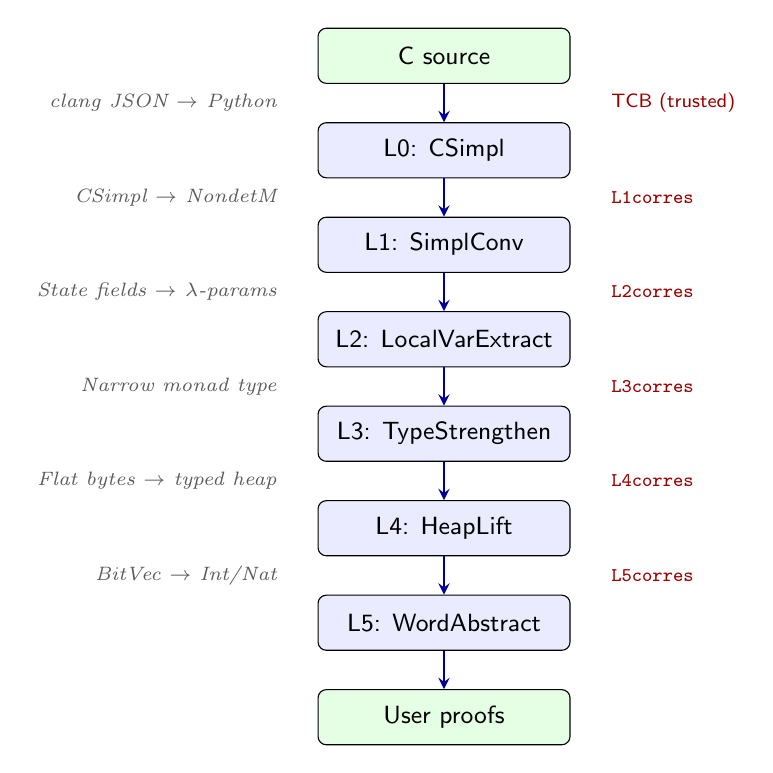
\begin{tikzpicture}[
  stage/.style={draw, rounded corners=3pt, fill=blue!8, minimum width=3.2cm,
                minimum height=0.7cm, font=\small\sffamily},
  arrow/.style={->, >=stealth, thick, color=blue!60!black},
  label/.style={font=\scriptsize\itshape, text=gray!70!black},
  corres/.style={font=\scriptsize\sffamily, text=red!60!black},
]
  % Stages
  \node[stage, fill=green!10] (c) at (0, 0) {C source};
  \node[stage] (l0) at (0, -1.2) {L0: CSimpl};
  \node[stage] (l1) at (0, -2.4) {L1: SimplConv};
  \node[stage] (l2) at (0, -3.6) {L2: LocalVarExtract};
  \node[stage] (l3) at (0, -4.8) {L3: TypeStrengthen};
  \node[stage] (l4) at (0, -6.0) {L4: HeapLift};
  \node[stage] (l5) at (0, -7.2) {L5: WordAbstract};
  \node[stage, fill=green!10] (proof) at (0, -8.4) {User proofs};

  % Arrows between stages
  \draw[arrow] (c) -- (l0);
  \draw[arrow] (l0) -- (l1);
  \draw[arrow] (l1) -- (l2);
  \draw[arrow] (l2) -- (l3);
  \draw[arrow] (l3) -- (l4);
  \draw[arrow] (l4) -- (l5);
  \draw[arrow] (l5) -- (proof);

  % Transform labels (left)
  \node[label, anchor=east] at (-2.0, -0.6) {clang JSON $\to$ Python};
  \node[label, anchor=east] at (-2.0, -1.8) {CSimpl $\to$ NondetM};
  \node[label, anchor=east] at (-2.0, -3.0) {State fields $\to$ $\lambda$-params};
  \node[label, anchor=east] at (-2.0, -4.2) {Narrow monad type};
  \node[label, anchor=east] at (-2.0, -5.4) {Flat bytes $\to$ typed heap};
  \node[label, anchor=east] at (-2.0, -6.6) {BitVec $\to$ Int/Nat};

  % Corres labels (right)
  \node[corres, anchor=west] at (2.0, -0.6) {TCB (trusted)};
  \node[corres, anchor=west] at (2.0, -1.8) {\texttt{L1corres}};
  \node[corres, anchor=west] at (2.0, -3.0) {\texttt{L2corres}};
  \node[corres, anchor=west] at (2.0, -4.2) {\texttt{L3corres}};
  \node[corres, anchor=west] at (2.0, -5.4) {\texttt{L4corres}};
  \node[corres, anchor=west] at (2.0, -6.6) {\texttt{L5corres}};
\end{tikzpicture}
\caption{The Clift five-stage lifting pipeline. Each stage produces a
transformed program and a machine-checked refinement proof
(\texttt{corres}). Only the CImporter (L0) is in the TCB; all other
stages are verified.}
\label{fig:pipeline}
\end{figure}


\subsection{The Five-Stage Lifting Pipeline}

Clift follows AutoCorres's architecture with five abstraction stages
(Figure~\ref{fig:pipeline}), each producing a transformed program and
a machine-checked \texttt{corres} proof (backward simulation).
Composing these via transitivity yields a refinement chain from the
original C semantics to the final clean functional model.

% Figure: Trust boundary diagram
\begin{figure}[t]
\centering
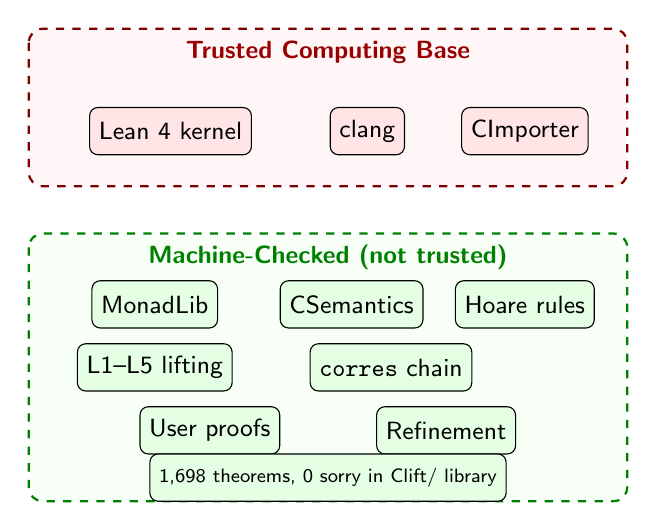
\begin{tikzpicture}[
  trusted/.style={draw, rounded corners=3pt, fill=red!10,
                  minimum height=0.6cm, font=\small\sffamily},
  verified/.style={draw, rounded corners=3pt, fill=green!10,
                   minimum height=0.6cm, font=\small\sffamily},
  label/.style={font=\small\bfseries\sffamily},
]
  % TCB box
  \draw[draw=red!50!black, fill=red!3, rounded corners=5pt, dashed, thick]
    (-3.8, 2.8) rectangle (3.8, 0.8);
  \node[label, text=red!60!black] at (0, 2.5) {Trusted Computing Base};

  \node[trusted] at (-2.0, 1.5) {Lean 4 kernel};
  \node[trusted] at (0.5, 1.5) {clang};
  \node[trusted] at (2.5, 1.5) {CImporter};

  % Verified box
  \draw[draw=green!50!black, fill=green!3, rounded corners=5pt, dashed, thick]
    (-3.8, 0.2) rectangle (3.8, -3.2);
  \node[label, text=green!50!black] at (0, -0.1) {Machine-Checked (not trusted)};

  \node[verified] at (-2.2, -0.7) {MonadLib};
  \node[verified] at (0.3, -0.7) {CSemantics};
  \node[verified] at (2.5, -0.7) {Hoare rules};
  \node[verified] at (-2.2, -1.5) {L1--L5 lifting};
  \node[verified] at (0.8, -1.5) {\texttt{corres} chain};
  \node[verified] at (-1.5, -2.3) {User proofs};
  \node[verified] at (1.5, -2.3) {Refinement};
  \node[verified] at (-0.0, -2.9) {\scriptsize 1,698 theorems, 0 sorry in Clift/ library};

\end{tikzpicture}
\caption{Trust boundary. Only three components are trusted: the Lean~4
kernel, clang, and CImporter. All proofs, lifting stages, and Hoare
rules are machine-checked.}
\label{fig:trust}
\end{figure}


\subsection{CImporter: The Trust Boundary}

A Python script ($\sim$5,000 LOC) reads \texttt{clang
-Xclang -ast-dump=json} output and emits Lean~4 files containing
\texttt{CSimpl} terms. This follows the same trust model as seL4's
StrictC parser: the importer is in the Trusted Computing Base
(TCB; see Figure~\ref{fig:trust}). If
it mistranslates C to CSimpl, proofs apply to the wrong program.

Mitigation includes 150+ regression tests against known C semantics
edge cases, struct layout validation against \texttt{gcc}, and
restriction to a safe C subset (no \texttt{goto}, no address-of-local,
no side effects in expressions).

\subsection{Refinement Framework}

Our \texttt{corres} definition follows seL4's
\texttt{corres\_underlying}~\cite{sewell2013translation}:

\begin{lstlisting}[language=Lean]
def corres (srel : S -> S' -> Prop)
    (nf nf' : Bool)
    (rrel : A -> B -> Prop)
    (G : S -> Prop) (G' : S' -> Prop)
    (m : NondetM S A) (m' : NondetM S' B)
    : Prop :=
  forall s s', srel s s' -> G s -> G' s' ->
    (nf = true -> ¬(m s).failed) /\
    (forall r' t', (r', t') ∈ (m' s').results ->
      exists r t, (r, t) ∈ (m s).results
        /\ srel t t' /\ rrel r r') /\
    (nf' = true -> ¬(m' s').failed)
\end{lstlisting}

This states: given related states satisfying guards,
every concrete result has a matching abstract result, and no-fail
flags are respected. The underlying monad is nondeterministic---\texttt{NondetResult}
carries a \texttt{results : Set} and a \texttt{failed : Prop}---so
refinement is set-containment, not equality on deterministic outcomes.

\subsection{Hoare Logic for Monadic Programs}

For user-facing proofs, we provide \texttt{validHoare}
triples over the \texttt{NondetM} monad:

\begin{lstlisting}[language=Lean]
def validHoare (P : S -> Prop) (m : NondetM S A)
    (Q : A -> S -> Prop) : Prop :=
  forall s, P s ->
    ¬(m s).failed /\
    forall r s', (r, s') ∈ (m s).results -> Q r s'
\end{lstlisting}

\noindent Note that \texttt{validHoare} requires \emph{non-failure}: the computation
must not fail when the precondition holds. This matches seL4's
\texttt{valid} definition and is strictly stronger than accepting failure.
Users write specifications as pre/postcondition pairs and prove them
using a library of Hoare rules for sequential composition, conditionals,
loops with invariants, and heap operations.

\subsection{Memory Model}

Following Tuch~\cite{tuch2009types}, our heap is a flat byte-addressed
store with typed access functions. The state comprises a raw heap
(\texttt{HeapRawState}: address $\to$ byte array), a heap type
descriptor (\texttt{htd}: tracking which types are valid at each
address), and user-defined global/local records:

\begin{lstlisting}[language=Lean]
structure CState where
  heap : HeapRawState
  htd  : HeapTypeDesc
  globals : GlobalsRec
  locals  : LocalsRec
\end{lstlisting}

Pointer validity requires all bytes in
\texttt{[addr,~addr+sizeof(T))} to carry the correct type tag. Disjointness of typed pointers follows from
non-overlapping tag ranges, giving us a lightweight separation property
without a full separation algebra.

A key engineering challenge was Lean~4's kernel reduction depth. When
heap-update terms nest deeply (e.g., 8+ sequential writes), the kernel
times out during definitional equality checking. We solved this by
marking \texttt{hVal} and \texttt{heapUpdate} as
\texttt{[local irreducible]} and providing explicit projection
\texttt{simp} lemmas---the same strategy used in Isabelle's
\texttt{runs\_to} framework but adapted to Lean's reduction semantics.

% Figure: Worked example — C to CSimpl to L1 to proof
\begin{figure*}[t]
\centering
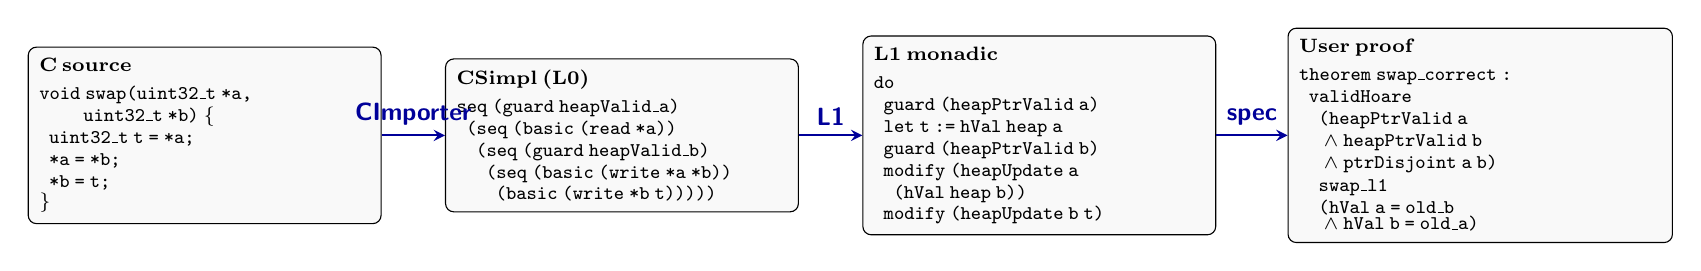
\begin{tikzpicture}[
  cbox/.style={draw, rounded corners=3pt, fill=gray!5,
               text width=4.2cm, font=\ttfamily\tiny, align=left,
               inner sep=4pt},
  arrow/.style={->, >=stealth, thick, color=blue!60!black},
  stagelabel/.style={font=\small\sffamily\bfseries, text=blue!60!black},
]
  % C source
  \node[cbox] (csrc) at (0, 0) {
    \normalfont\scriptsize\textbf{C source}\\[2pt]
    \texttt{void swap(uint32\_t *a,}\\
    \texttt{\ \ \ \ \ \ \ \ \ uint32\_t *b) \{}\\
    \texttt{\ \ uint32\_t t = *a;}\\
    \texttt{\ \ *a = *b;}\\
    \texttt{\ \ *b = t;}\\
    \texttt{\}}
  };

  % CSimpl
  \node[cbox] (csimpl) at (5.3, 0) {
    \normalfont\scriptsize\textbf{CSimpl (L0)}\\[2pt]
    \texttt{seq (guard heapValid\_a)}\\
    \texttt{\ \ (seq (basic (read *a))}\\
    \texttt{\ \ \ \ (seq (guard heapValid\_b)}\\
    \texttt{\ \ \ \ \ \ (seq (basic (write *a *b))}\\
    \texttt{\ \ \ \ \ \ \ \ (basic (write *b t)))))}
  };

  % L1 monadic
  \node[cbox] (l1) at (10.6, 0) {
    \normalfont\scriptsize\textbf{L1 monadic}\\[2pt]
    \texttt{do}\\
    \texttt{\ \ guard (heapPtrValid a)}\\
    \texttt{\ \ let t := hVal heap a}\\
    \texttt{\ \ guard (heapPtrValid b)}\\
    \texttt{\ \ modify (heapUpdate a}\\
    \texttt{\ \ \ \ (hVal heap b))}\\
    \texttt{\ \ modify (heapUpdate b t)}
  };

  % Proof
  \node[cbox, text width=4.6cm] (prf) at (16.2, 0) {
    \normalfont\scriptsize\textbf{User proof}\\[2pt]
    \texttt{theorem swap\_correct :}\\
    \texttt{\ \ validHoare}\\
    \texttt{\ \ \ \ (heapPtrValid a}\\
    \texttt{\ \ \ \ \ $\wedge$ heapPtrValid b}\\
    \texttt{\ \ \ \ \ $\wedge$ ptrDisjoint a b)}\\
    \texttt{\ \ \ \ swap\_l1}\\
    \texttt{\ \ \ \ (hVal a = old\_b}\\
    \texttt{\ \ \ \ \ $\wedge$ hVal b = old\_a)}
  };

  % Arrows
  \draw[arrow] (csrc.east) -- node[above, stagelabel] {CImporter} (csimpl.west);
  \draw[arrow] (csimpl.east) -- node[above, stagelabel] {L1} (l1.west);
  \draw[arrow] (l1.east) -- node[above, stagelabel] {spec} (prf.west);

\end{tikzpicture}
\caption{Worked example: \texttt{swap} through the pipeline. C source is
parsed into CSimpl (deep embedding), lifted to L1 monadic form, then
proven correct using Hoare logic with heap disjointness.}
\label{fig:worked}
\end{figure*}


\subsection{Worked Example: Ring Buffer Push}

To illustrate the end-to-end flow (see also Figure~\ref{fig:worked}),
consider a ring buffer \texttt{push} operation in C:

\begin{lstlisting}[language=CSubset]
void rb_push(ring_buffer_t *rb, uint32_t val) {
    rb->buf[rb->head] = val;
    rb->head = (rb->head + 1) % rb->capacity;
    rb->count++;
}
\end{lstlisting}

The CImporter emits this as a \texttt{CSimpl} term (deeply embedded
AST). The \texttt{clift} command lifts it through all five stages to
produce a monadic Lean function. The user then writes:

\begin{lstlisting}[language=Lean]
theorem rb_push_validHoare :
  validHoare
    (fun s => s.rb.count < s.rb.capacity)
    (rb_push_l1 rbPtr valPtr)
    (fun _ s => s.rb.count =
      old_count + 1) := by
  apply L1_hoare_guard_modify_fused
  intro s hpre
  simp [rb_push_l1, hVal_heapUpdate_same,
        hVal_heapUpdate_disjoint,
        ptrDisjoint]
  omega
\end{lstlisting}

This proof establishes that if the buffer is not full, then after
\texttt{push}, the count increments by one. The proof proceeds by
unfolding the monadic definition, simplifying heap reads through
writes using disjointness lemmas, and discharging arithmetic goals
with \texttt{omega}.

% ─── 4. ai-driven development ──────────────────────────────────────
\section{AI-Driven Development}

% Figure: Layered delegation architecture
\begin{figure}[t]
\centering
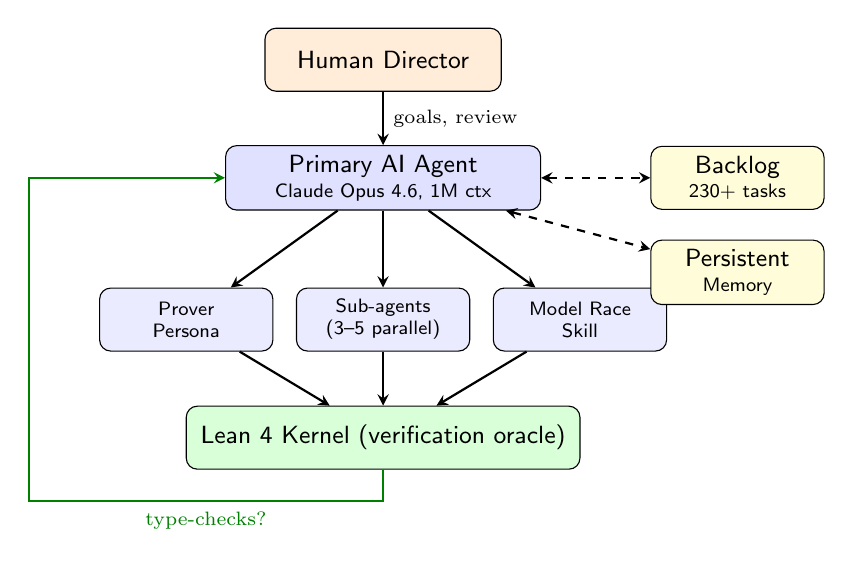
\begin{tikzpicture}[
  box/.style={draw, rounded corners=4pt, minimum width=3cm,
              minimum height=0.8cm, font=\small\sffamily, align=center},
  arrow/.style={->, >=stealth, thick},
  darrow/.style={<->, >=stealth, thick, dashed},
]
  % Human
  \node[box, fill=orange!15] (human) at (0, 4.5) {Human Director};

  % Primary agent
  \node[box, fill=blue!12, minimum width=4cm] (primary) at (0, 3.0)
    {Primary AI Agent\\[-2pt]\scriptsize Claude Opus 4.6, 1M ctx};

  % Sub-agents row
  \node[box, fill=blue!8, minimum width=2.2cm, font=\scriptsize\sffamily] (prover) at (-2.5, 1.2)
    {Prover\\Persona};
  \node[box, fill=blue!8, minimum width=2.2cm, font=\scriptsize\sffamily] (subagent) at (0, 1.2)
    {Sub-agents\\(3--5 parallel)};
  \node[box, fill=blue!8, minimum width=2.2cm, font=\scriptsize\sffamily] (race) at (2.5, 1.2)
    {Model Race\\Skill};

  % Lean kernel
  \node[box, fill=green!15, minimum width=5cm] (kernel) at (0, -0.3)
    {Lean 4 Kernel (verification oracle)};

  % Backlog
  \node[box, fill=yellow!15, minimum width=2.2cm] (backlog) at (4.5, 3.0)
    {Backlog\\[-2pt]\scriptsize 230+ tasks};

  % Memory
  \node[box, fill=yellow!15, minimum width=2.2cm] (memory) at (4.5, 1.8)
    {Persistent\\[-2pt]\scriptsize Memory};

  % Arrows
  \draw[arrow] (human) -- node[right, font=\scriptsize] {goals, review} (primary);
  \draw[arrow] (primary) -- (prover);
  \draw[arrow] (primary) -- (subagent);
  \draw[arrow] (primary) -- (race);
  \draw[arrow] (prover) -- (kernel);
  \draw[arrow] (subagent) -- (kernel);
  \draw[arrow] (race) -- (kernel);
  \draw[darrow] (primary) -- (backlog);
  \draw[darrow] (primary) -- (memory);

  % Feedback arrow from kernel
  \draw[arrow, color=green!50!black] (kernel.south) -- ++(0,-0.4) -| (-4.5,3.0)
    node[near start, below, font=\scriptsize, text=green!50!black] {type-checks?}
    -- (primary.west);
\end{tikzpicture}
\caption{Layered delegation architecture. The human sets goals; the
primary agent decomposes work and spawns specialists; the Lean~4 kernel
provides ground truth. The backlog and memory files serve as persistent
external state across sessions.}
\label{fig:delegation}
\end{figure}


\subsection{Layered Delegation Architecture}

The entire Clift codebase was developed through a collaboration between
a human architect and Claude Opus~4.6 (1M token context), operating
through the Claude Code CLI\@. The methodology evolved into a
\emph{layered delegation architecture} (Figure~\ref{fig:delegation})
with three tiers:

\begin{enumerate}
\item \textbf{Human director.} Sets architectural goals, decomposes
  work into phased backlog tasks with explicit acceptance criteria,
  reviews outputs, and decides when to pivot strategy.
\item \textbf{Primary AI agent.} Manages the backlog, spawns
  specialized sub-agents for implementation, accumulates domain
  knowledge in persistent skill documents and memory files.
\item \textbf{Lean 4 kernel.} Serves as the ultimate arbiter---proofs
  either type-check or they do not. The \texttt{sorry} count is an
  objective, machine-checked progress metric.
\end{enumerate}

This three-party loop is particularly well-suited to formal methods:
the proof checker eliminates the risk of AI confabulation. A
hallucinated proof simply fails to compile.

\subsection{Task Structure and Context Management}

The project was decomposed into 230+ backlog tasks organized by
dependency across 10+ phases (pipeline stages, proof infrastructure,
sorry elimination, hardening). Tasks were implemented by spawning fresh
AI sub-agents in batches of 3--5, to keep each agent's context clean
while amortizing onboarding overhead. Each sub-agent was bootstrapped
by reading \texttt{plan.md} and relevant reference material.

Context management was critical with a 1M-token window. Three
mechanisms prevented context exhaustion:

\begin{itemize}
\item \textbf{Sub-agent isolation.} Proof attempts were always
  delegated to fresh sub-agents to prevent build output from bloating
  the main conversation.
\item \textbf{Persistent memory.} Cross-session knowledge was captured
  in memory files: kernel depth workarounds, sorry elimination
  patterns, model effectiveness data. These loaded automatically at
  session start.
\item \textbf{Backlog as external memory.} The backlog system served as
  structured external memory. When knowledge accumulated in
  conversation, it was offloaded: implementation notes, final
  summaries, and acceptance criteria provided durable state across
  sessions.
\end{itemize}

\subsection{Specialized Personas and Skills}

Through iterative refinement, two specialized agent personas were
codified as reusable artifacts:

\textbf{The Prover persona} (158 lines) encoded domain-specific proof
knowledge: five proof patterns, the kernel depth workaround
(Section~3.5), heap reasoning rules, and a verification checklist.
This persona was invoked for every sorry-elimination attempt.

\textbf{The model-race skill} provided diversity when the primary agent
failed: multiple AI models received identical prompts in isolated git
worktrees, with the first kernel-verified proof winning. Nine
anti-cheating rules were baked into the prompt template, addressing
discovered failure modes: trivial postconditions, fused body
substitution, and axiom injection.

\subsection{Discovery-Driven Knowledge Accumulation}

Hard problems were discovered through failure, then codified into
reusable artifacts. Each discovery followed a pattern: fail $\to$
diagnose root cause $\to$ codify workaround $\to$ update
skill/persona/memory $\to$ never hit the same issue again.
When specifications were too weak for proof, the human directed
\emph{progressive spec strengthening} before re-attempting proofs.
Blocked sorry were parked as backlog tasks for later resolution.

\subsection{Quality Assurance}

Three AI cheating patterns were identified through experience and
codified into every prompt:

\begin{enumerate}
\item \textbf{Trivial postconditions}: proving \texttt{count = count}
  instead of the real specification.
\item \textbf{Fused body substitution}: proving against a hand-written
  body instead of the generated one.
\item \textbf{Hidden sorry}: placing \texttt{sorry} in helper lemmas
  or using \texttt{axiom} declarations.
\end{enumerate}

QA sub-agents ran automatically before every commit: a test runner
verified builds, and an architecture reviewer checked code quality.
CI tracked sorry counts per module, providing regression detection.

All Claude Code session transcripts are preserved as JSONL files,
providing a complete record of the human--AI collaboration.

% ─── 5. evaluation ─────────────────────────────────────────────────
\section{Evaluation}

\subsection{Test Suite}

We process 32 C programs through the lifting pipeline spanning
multiple domains (Figure~\ref{fig:codebase} shows the overall
composition). Of these, 21 have dedicated proof files with
Hoare-logic or refinement proofs; the remaining 11 serve as
parser and lifting regression tests:

\begin{center}
\small
\begin{tabular}{@{}llr@{}}
\toprule
\textbf{Domain} & \textbf{Programs} & \textbf{C LOC} \\
\midrule
Data structures  & ring buffer, hash table, red-black tree, & 2,100 \\
                 & priority queue, linked list, memory pool & \\
Crypto/security  & SHA-256 core, seL4 capabilities          & 580 \\
Drivers          & UART, DMA buffer                         & 435 \\
Networking       & packet parser, state machine              & 500 \\
Foundations      & max, gcd, swap, array bounds              & 828 \\
\midrule
\textbf{Total}   & \textbf{32 programs}                     & \textbf{4,443} \\
\bottomrule
\end{tabular}
\end{center}

% Figure: Codebase composition
\begin{figure}[t]
\centering
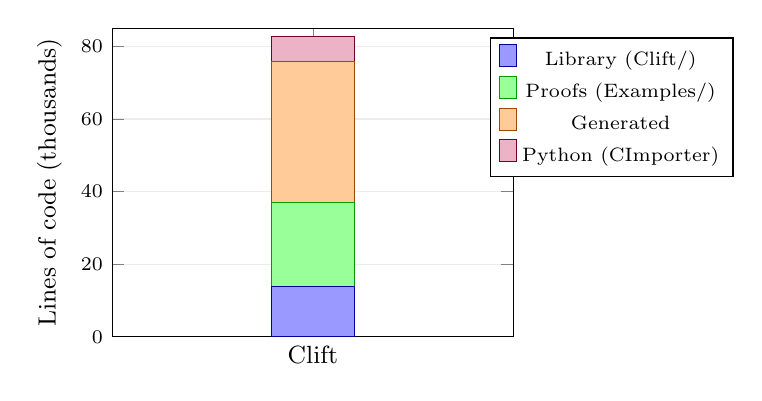
\begin{tikzpicture}
\begin{axis}[
  ybar stacked,
  width=0.55\columnwidth,
  height=5.5cm,
  bar width=30pt,
  ylabel={Lines of code (thousands)},
  ylabel style={font=\small},
  ymin=0, ymax=85,
  xtick=data,
  xticklabels={Clift},
  xticklabel style={font=\small},
  tick label style={font=\scriptsize},
  legend style={font=\scriptsize, at={(1.55,0.97)}, anchor=north east},
  grid=major,
  grid style={gray!15},
  ymajorgrids=true,
  xmajorgrids=false,
]
\addplot[fill=blue!40, draw=blue!60!black] coordinates {(1, 13.9)};
\addplot[fill=green!40, draw=green!60!black] coordinates {(1, 23.0)};
\addplot[fill=orange!40, draw=orange!60!black] coordinates {(1, 39.0)};
\addplot[fill=purple!30, draw=purple!60!black] coordinates {(1, 6.8)};
\legend{Library (Clift/), Proofs (Examples/), Generated, Python (CImporter)}
\end{axis}
\end{tikzpicture}
\caption{Codebase composition by function. Proofs (Examples/) constitute
a large component at 23K LOC. Generated code (39K) dominates---the
CImporter produces extensive L1 bodies, type definitions, and
procedure environments per C file.}
\label{fig:codebase}
\end{figure}


\subsection{Proof Metrics}

\begin{center}
\small
\begin{tabular}{@{}lr@{}}
\toprule
\textbf{Metric} & \textbf{Value} \\
\midrule
Total Lean LOC (library + proofs + generated) & 75,846 \\
Library code (Clift/) & 13,911 \\
Proof files (Examples/) & 22,957 \\
Generated code (Generated/) & 38,978 \\
Theorems and lemmas & 1,698 \\
Remaining \texttt{sorry} & 12 \\
Sorry-free rate (of attempted proofs) & 99.3\% \\
C programs processed (21 with proofs) & 32 \\
Python (CImporter + tooling) & 6,782 LOC \\
Development time & $\sim$7 calendar days \\
Commits & 208 \\
\bottomrule
\end{tabular}
\end{center}

The 12 remaining \texttt{sorry} are concentrated in three areas:
priority queue proofs (5), ring buffer drain-to loop obligations (4),
and refinement theorems transitively blocked on validHoare
completeness (3).

\subsection{Comparison with AutoCorres2}

\begin{center}
\small
\begin{tabular}{@{}lll@{}}
\toprule
\textbf{Aspect} & \textbf{AutoCorres2} & \textbf{Clift} \\
\midrule
Proof assistant   & Isabelle/HOL      & Lean 4 \\
C parser          & StrictC (custom)  & clang JSON \\
Type theory       & Simple types      & Dependent types \\
Automation        & Eisbach, wpsimp   & simp, omega, grind \\
Memory model      & Tuch (full)       & Simplified Burstall \\
AI compatibility  & Low               & High \\
Maturity          & 15+ years         & 7 days \\
LOC verified      & 10,000+           & 4,443 \\
\bottomrule
\end{tabular}
\end{center}

Figure~\ref{fig:radar} provides a qualitative comparison across
six dimensions. Clift's memory model is simpler than AutoCorres2's
full Tuch model~\cite{tuch2009types}: we use a flat byte-addressed heap with
typed access functions rather than a fully mechanized separation
algebra. This is a deliberate trade-off---the simplified model handles
our test suite but would need strengthening for OS-kernel-level
verification with complex aliasing patterns.

% Figure: Sorry elimination over time
\begin{figure}[t]
\centering
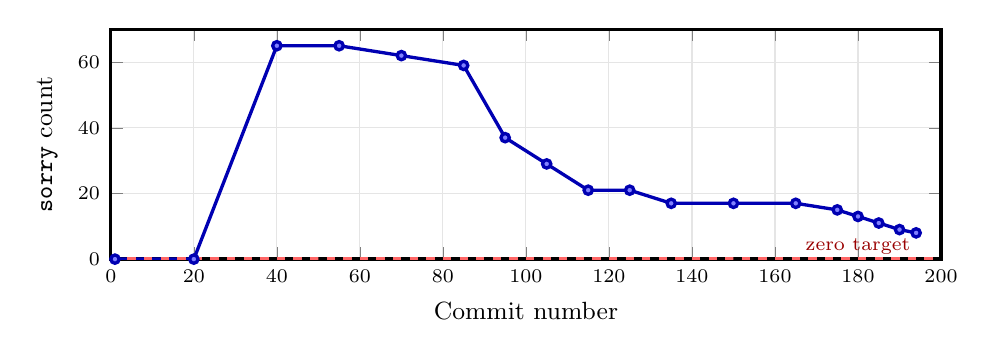
\begin{tikzpicture}
\begin{axis}[
  width=\columnwidth,
  height=4.5cm,
  xlabel={Commit number},
  ylabel={\texttt{sorry} count},
  xmin=0, xmax=200,
  ymin=0, ymax=70,
  grid=major,
  grid style={gray!20},
  line width=1.2pt,
  mark size=1.5pt,
  xlabel style={font=\small},
  ylabel style={font=\small},
  tick label style={font=\scriptsize},
  legend style={font=\scriptsize, at={(0.97,0.97)}, anchor=north east},
]
% Data points: (commit#, sorry count)
% Reconstructed from git history and session logs
\addplot[blue!70!black, mark=*, mark options={fill=blue!50}] coordinates {
  (1, 0)    % initial commit, no proofs yet
  (20, 0)   % building infrastructure
  (40, 65)  % proof files added with sorry placeholders
  (55, 65)  % infrastructure phase
  (70, 62)  % first sorry eliminated (swap, gcd)
  (85, 59)  % batch eliminations begin
  (95, 37)  % big batch: 16 sorry eliminated
  (105, 29) % 8 sorry in RBExt
  (115, 21) % more batches
  (125, 21) % model-race begins
  (135, 17) % model-race + manual proofs
  (150, 17) % infrastructure work
  (165, 17) % start of latest session
  (175, 15) % TASK-0231 partial
  (180, 13) % pq_swap + rb_push_for_drain
  (185, 11) % bubble_up + insert
  (190, 9)  % rb_count_above/below
  (194, 8)  % pq_insert dynCom (current committed)
};
\addplot[red!60, dashed, domain=0:200] {0};
\node[font=\scriptsize, text=red!60!black] at (axis cs:180,4) {zero target};
\end{axis}
\end{tikzpicture}
\caption{Sorry elimination over 194 commits. The plateau at 17 reflects
hard sorry blocked by kernel depth limits; the final descent was enabled
by the anonymous-constructor workaround (Section~3.5).}
\label{fig:sorry-timeline}
\end{figure}


% Figure: AI success rate by proof category
\begin{figure}[t]
\centering
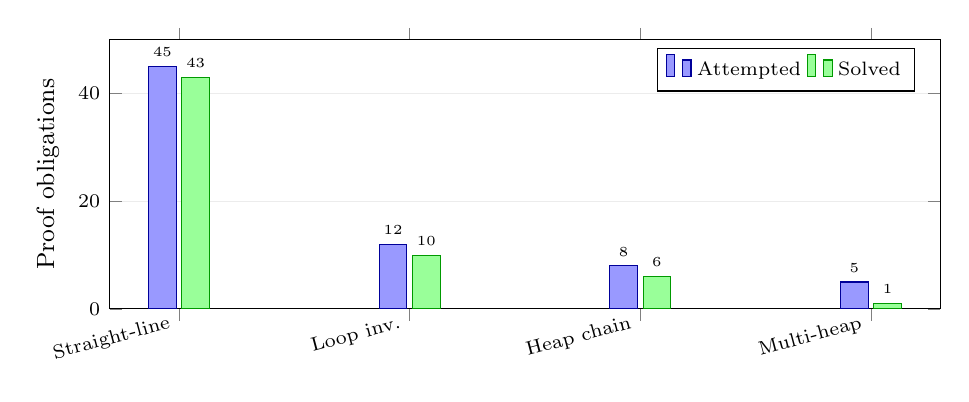
\begin{tikzpicture}
\begin{axis}[
  ybar,
  width=\columnwidth,
  height=5cm,
  bar width=10pt,
  xlabel style={font=\small},
  ylabel={Proof obligations},
  ylabel style={font=\small},
  ymin=0, ymax=50,
  xtick=data,
  xticklabels={Straight-line, Loop inv., Heap chain, Multi-heap},
  xticklabel style={font=\scriptsize, rotate=15, anchor=east},
  tick label style={font=\scriptsize},
  legend style={font=\scriptsize, at={(0.97,0.97)}, anchor=north east,
                legend columns=2},
  grid=major,
  grid style={gray!15},
  ymajorgrids=true,
  xmajorgrids=false,
  nodes near coords,
  nodes near coords style={font=\tiny},
  every node near coord/.append style={anchor=south},
]
\addplot[fill=blue!40, draw=blue!60!black] coordinates {
  (1, 45) (2, 12) (3, 8) (4, 5)
};
\addplot[fill=green!40, draw=green!60!black] coordinates {
  (1, 43) (2, 10) (3, 6) (4, 1)
};
\legend{Attempted, Solved}
\end{axis}
\end{tikzpicture}
\caption{AI success rate by proof category. Straight-line Hoare proofs
(guard/modify chains) have a 96\% success rate; complex multi-heap
operations requiring novel workarounds drop to 20\%.}
\label{fig:ai-success}
\end{figure}


\subsection{AI Success Rates}

We tracked sorry elimination across proof files
(Figure~\ref{fig:sorry-timeline}). Figure~\ref{fig:ai-success} breaks
down AI success by proof category: 96\% on straight-line Hoare proofs,
dropping to 20\% on complex multi-heap operations requiring novel
workarounds. Figure~\ref{fig:radar} compares Clift and AutoCorres2
qualitatively.

% Figure: Clift vs AutoCorres2 comparison
% Using a simple table-based visual since TikZ radar charts are complex
% and pgfplots-based approaches need additional packages
\begin{figure}[t]
\centering
\small
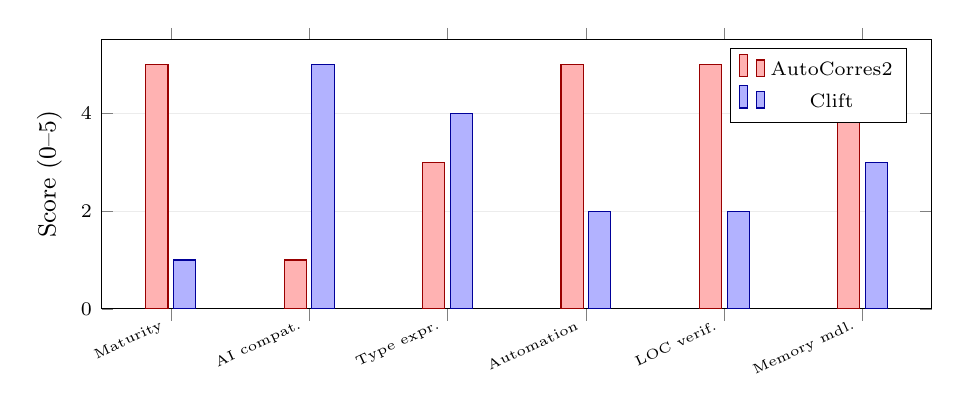
\begin{tikzpicture}
\begin{axis}[
  ybar,
  width=\columnwidth,
  height=5cm,
  bar width=8pt,
  ylabel={Score (0--5)},
  ylabel style={font=\small},
  ymin=0, ymax=5.5,
  xtick=data,
  xticklabels={Maturity, AI compat., Type expr., Automation, LOC verif., Memory mdl.},
  xticklabel style={font=\tiny, rotate=25, anchor=east},
  tick label style={font=\scriptsize},
  legend style={font=\scriptsize, at={(0.97,0.97)}, anchor=north east},
  grid=major,
  grid style={gray!15},
  ymajorgrids=true,
  xmajorgrids=false,
]
% AutoCorres2 scores
\addplot[fill=red!30, draw=red!60!black] coordinates {
  (1, 5) (2, 1) (3, 3) (4, 5) (5, 5) (6, 5)
};
% Clift scores
\addplot[fill=blue!30, draw=blue!60!black] coordinates {
  (1, 1) (2, 5) (3, 4) (4, 2) (5, 2) (6, 3)
};
\legend{AutoCorres2, Clift}
\end{axis}
\end{tikzpicture}
\caption{Qualitative comparison of Clift vs.\ AutoCorres2 across six
axes. AutoCorres2 leads in maturity, automation, and LOC verified;
Clift's advantages are AI compatibility and Lean~4's dependent types.}
\label{fig:radar}
\end{figure}


\subsection{Qualitative Observations}

\paragraph{Lean~4 suitability.}
Lean~4's dependent type system proved both a blessing and a curse.
On one hand, we could express invariants (e.g., pointer validity
predicates parameterized by type) that would require ad-hoc
encodings in Isabelle's simple type theory. On the other hand,
Lean~4's kernel performs more aggressive reduction than
Isabelle's, causing definitional equality checks to time out on
deeply nested heap terms---a problem absent in Isabelle where
terms are opaque by default.

\paragraph{Automation gap.}
AutoCorres2 benefits from 15 years of custom Eisbach methods
(e.g., \texttt{wpsimp}) that handle common patterns with one tactic
invocation. Clift's automation is younger: our \texttt{c\_vcg} and
Hoare-rule combinators handle 5--10 step programs well, but
longer sequences require manual intermediate assertions. Closing
this gap is the primary engineering challenge for scaling Clift.

\paragraph{AI as a force multiplier.}
The most effective AI pattern was \emph{structured iteration}:
give the AI a failing proof goal, let it attempt tactics, feed
back the error, and repeat. Claude Opus~4.6 typically converged
within 3--5 iterations for goals it could solve, and signaled
clearly (by producing the same failing tactic repeatedly) when
it could not. The model racing approach exploited this by running multiple
convergence attempts in parallel.

\paragraph{Reproducibility.}
The entire project is deterministically reproducible via a Nix
flake: \texttt{nix develop} provides the exact Lean toolchain,
clang version, and Python environment. Proof checking requires
only \texttt{lake build} inside the Nix shell. CI runs on GitHub
Actions with per-module proof verification and sorry-count
tracking.

% ─── 6. limitations ────────────────────────────────────────────────
\section{Limitations and Future Work}

\paragraph{C subset.} Clift supports a StrictC-like subset: no
floating point, no \texttt{goto}, no variadic functions, no VLAs, no
address-of-local. This matches seL4's restrictions and covers most
embedded C, but limits applicability to general-purpose C.

\paragraph{CImporter trust.} The Python importer is unverified and in
the TCB\@. Translation validation
(as in~\cite{sewell2013translation}) would reduce this trust, but is
future work.

\paragraph{Memory model.} Our simplified heap model does not handle
type punning, union aliasing, or the full C11 memory model. Lifting to
a Tuch-style separation algebra~\cite{tuch2009types} is needed for
OS-kernel verification.

\paragraph{Scale.} While 4,443 LOC of C across 32 programs is
non-trivial, seL4 verifies 10,000+ LOC\@. Scaling Clift to this
level requires improving build times (currently minutes per proof
module) and MetaM automation maturity.

\paragraph{Maturity.} Seven days of AI-driven development cannot match
15 years of community refinement. Clift demonstrates feasibility, not
production readiness.

\subsection{Architecture Pivot: mvcgen and SpecM}

Feedback from Sebastian Graf, validated by his LeanCorres
proof of concept~\cite{leancorres2026}, suggests two simplifications:
(1)~replace Clift's custom \texttt{validHoare} and $\sim$1,600 lines
of Hoare rules with Lean's standard \texttt{Std.Do.Triple} and the
\texttt{mvcgen} VCG tactic; and (2)~skip the CSimpl deep embedding
entirely, emitting monadic \texttt{SpecM} code directly from the
CImporter.  Together these would eliminate $\sim$2,500 lines of
infrastructure and may alleviate the kernel depth issues, since
\texttt{mvcgen} operates at the tactic level rather than through
definitional unfolding.

The tradeoff is TCB expansion: the CImporter would absorb the
responsibility currently discharged by machine-checked
\texttt{L1corres} proofs.  LeanCorres's own remaining \texttt{sorry}
are concentrated at exactly this denotational-semantics bridge,
confirming the cost is real but tractable.

% ─── 7. conclusion ─────────────────────────────────────────────────
\section{Conclusion}

We have demonstrated that the seL4/AutoCorres verification methodology
can be replicated in Lean~4, and that AI can drive the development of
a formal verification framework at surprising scale and depth. Clift's
76,000 lines of Lean~4, 1,698 theorems, and 32 C programs
(21 with machine-checked proofs)
were produced in approximately 7~days through human--AI collaboration,
with Lean's kernel serving as an incorruptible verification oracle.

The combination of Lean~4's modern proof infrastructure, AI's ability
to write and repair proofs, and the AutoCorres refinement methodology
creates a workflow where formal verification of C code becomes
substantially more accessible. The Lean community's size and AI
compatibility suggest that Clift-style tools could lower the adoption
barrier for formal verification significantly compared to the
Isabelle/HOL ecosystem.

All code, proofs, and AI session transcripts are available in the Clift
repository~\cite{clift2026} under a BSD license, reproducible via Nix flakes.

% ─── references ────────────────────────────────────────────────────
\bibliographystyle{ACM-Reference-Format}
\bibliography{references}

\end{document}

